%==============================================================================
%  APPENDICES
%  Each \chapter here is numbered A, B, C, ... because thesis.tex issues
%  \appendix before \include-ing this file.
%==============================================================================
\graphicspath{{Appendix_folder/PLOTS/}}

\chapter{Merger posterior distributions of MW accreted substructures}
\label{app:A}

This appendix supplements Chapter~\ref{chap:chapter5}. The posterior distributions of the lookback infall time, stellar and halo mass, and halo mass merger ratio of the MW accreted satellites were estimated from the present-day chemodynamics of their debris using an ensemble of Masked Autoregressive Flows following the GalactiKit methodology. In Chapter~\ref{chap:chapter5}, samples from these distributions were used to compute summary statistics, providing a quantitative description of the properties of each merger event and, overall, of the MW assembly history.

In this section, the posterior sample distributions for the accreted substructures are reported in individual figures: GES (Fig.~\ref{fig:GES_pdf}), Helmi streams (Fig.~\ref{fig:Helmi_pdf}), Heracles (Fig.~\ref{fig:Heracles_pdf}), I'itoi (Fig.~\ref{fig:Iitoi_pdf}), LMS-1/Wukong (Fig.~\ref{fig:LMS_pdf}), Sagittarius (Fig.~\ref{fig:Sagittarius_pdf}), and Thamnos (Fig.~\ref{fig:Thamnos_pdf}). For Sequoia, we provide three distributions conditioned on debris selected with different criteria: \textit{K19} (Fig.~\ref{fig:Sequoia_K19_pdf}), \textit{M19} (Fig.~\ref{fig:Sequoia_M19_pdf}), and \textit{N20} (Fig.~\ref{fig:Sequoia_N20_pdf}). Each distribution is presented as a corner plot of the inferred galaxy merger properties, with one-dimensional density distributions showing the median and the 16th--84th percentile range. Samples are coloured consistently with the substructure colour scheme adopted in the analysis.


\begin{figure*}
    \centering
    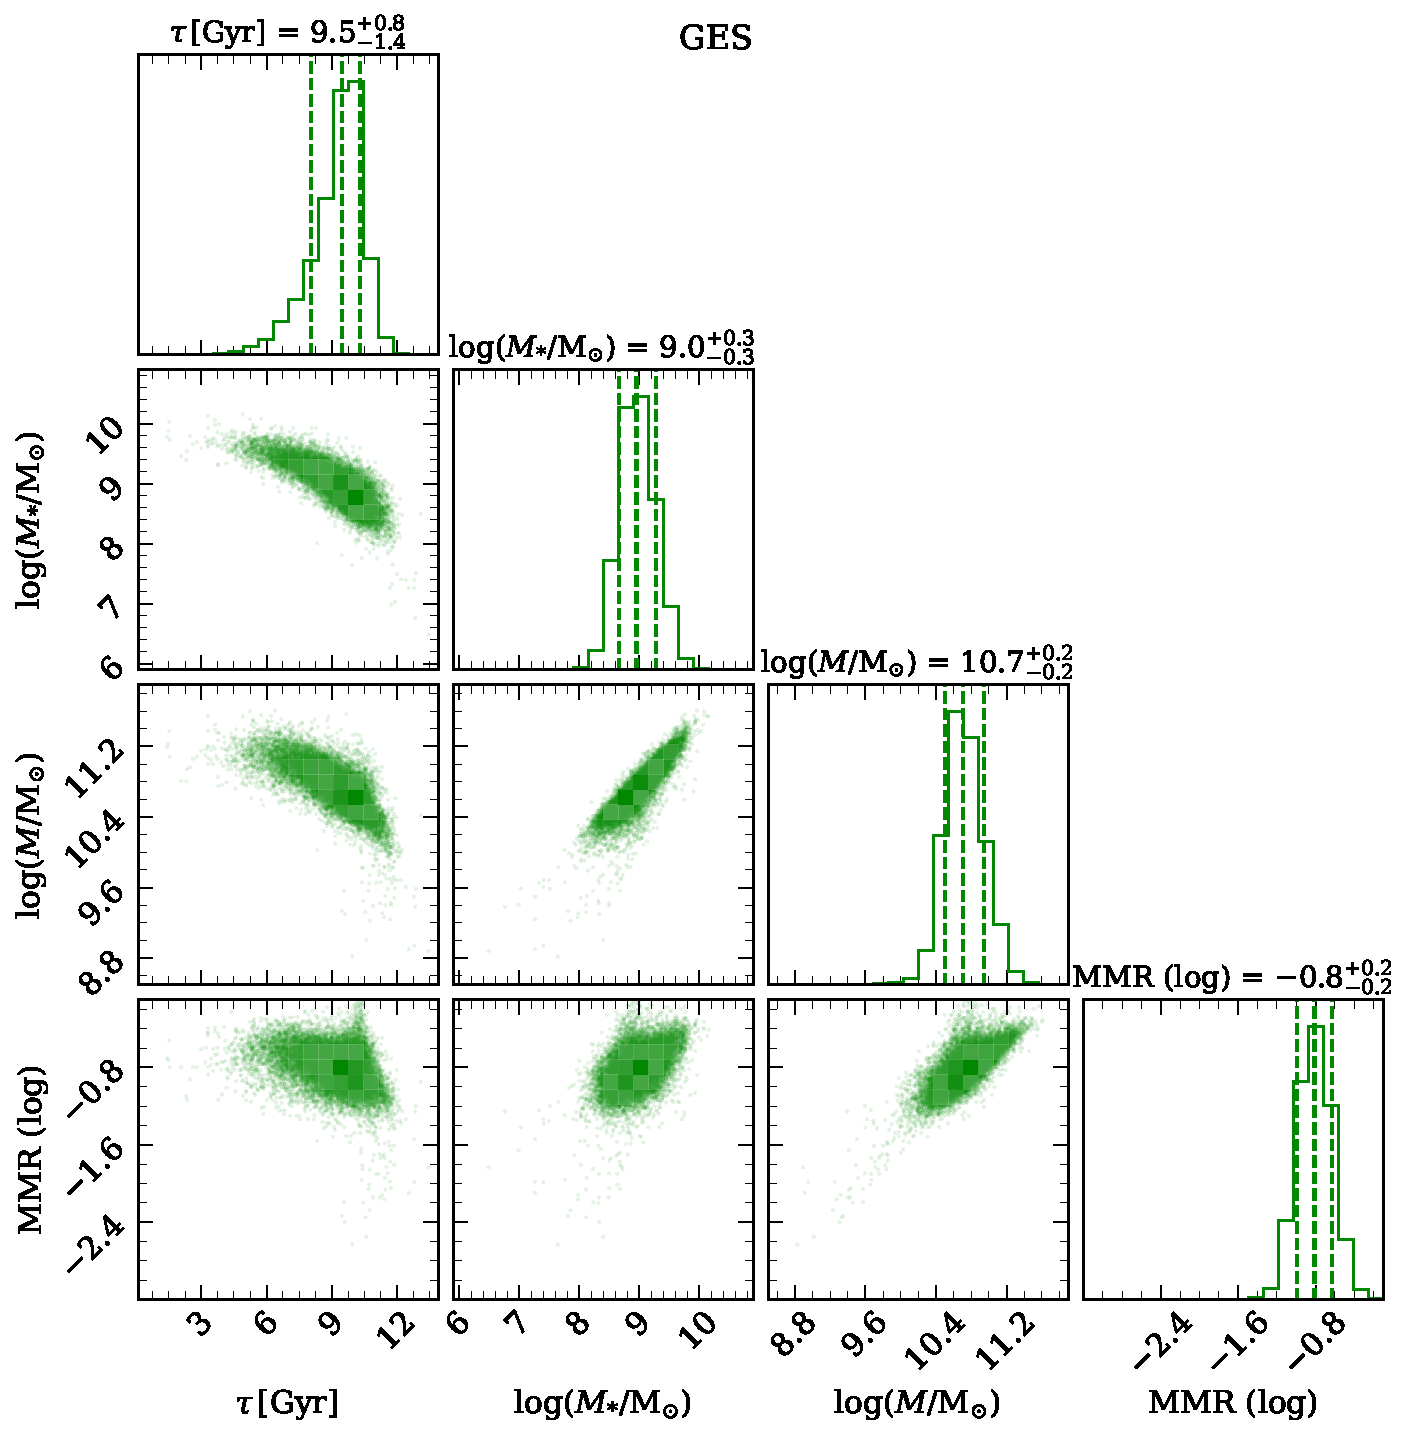
\includegraphics[width=\linewidth]{GES.pdf}
    \caption{}
    \label{fig:GES_pdf}
\end{figure*}


\begin{figure*}
    \centering
    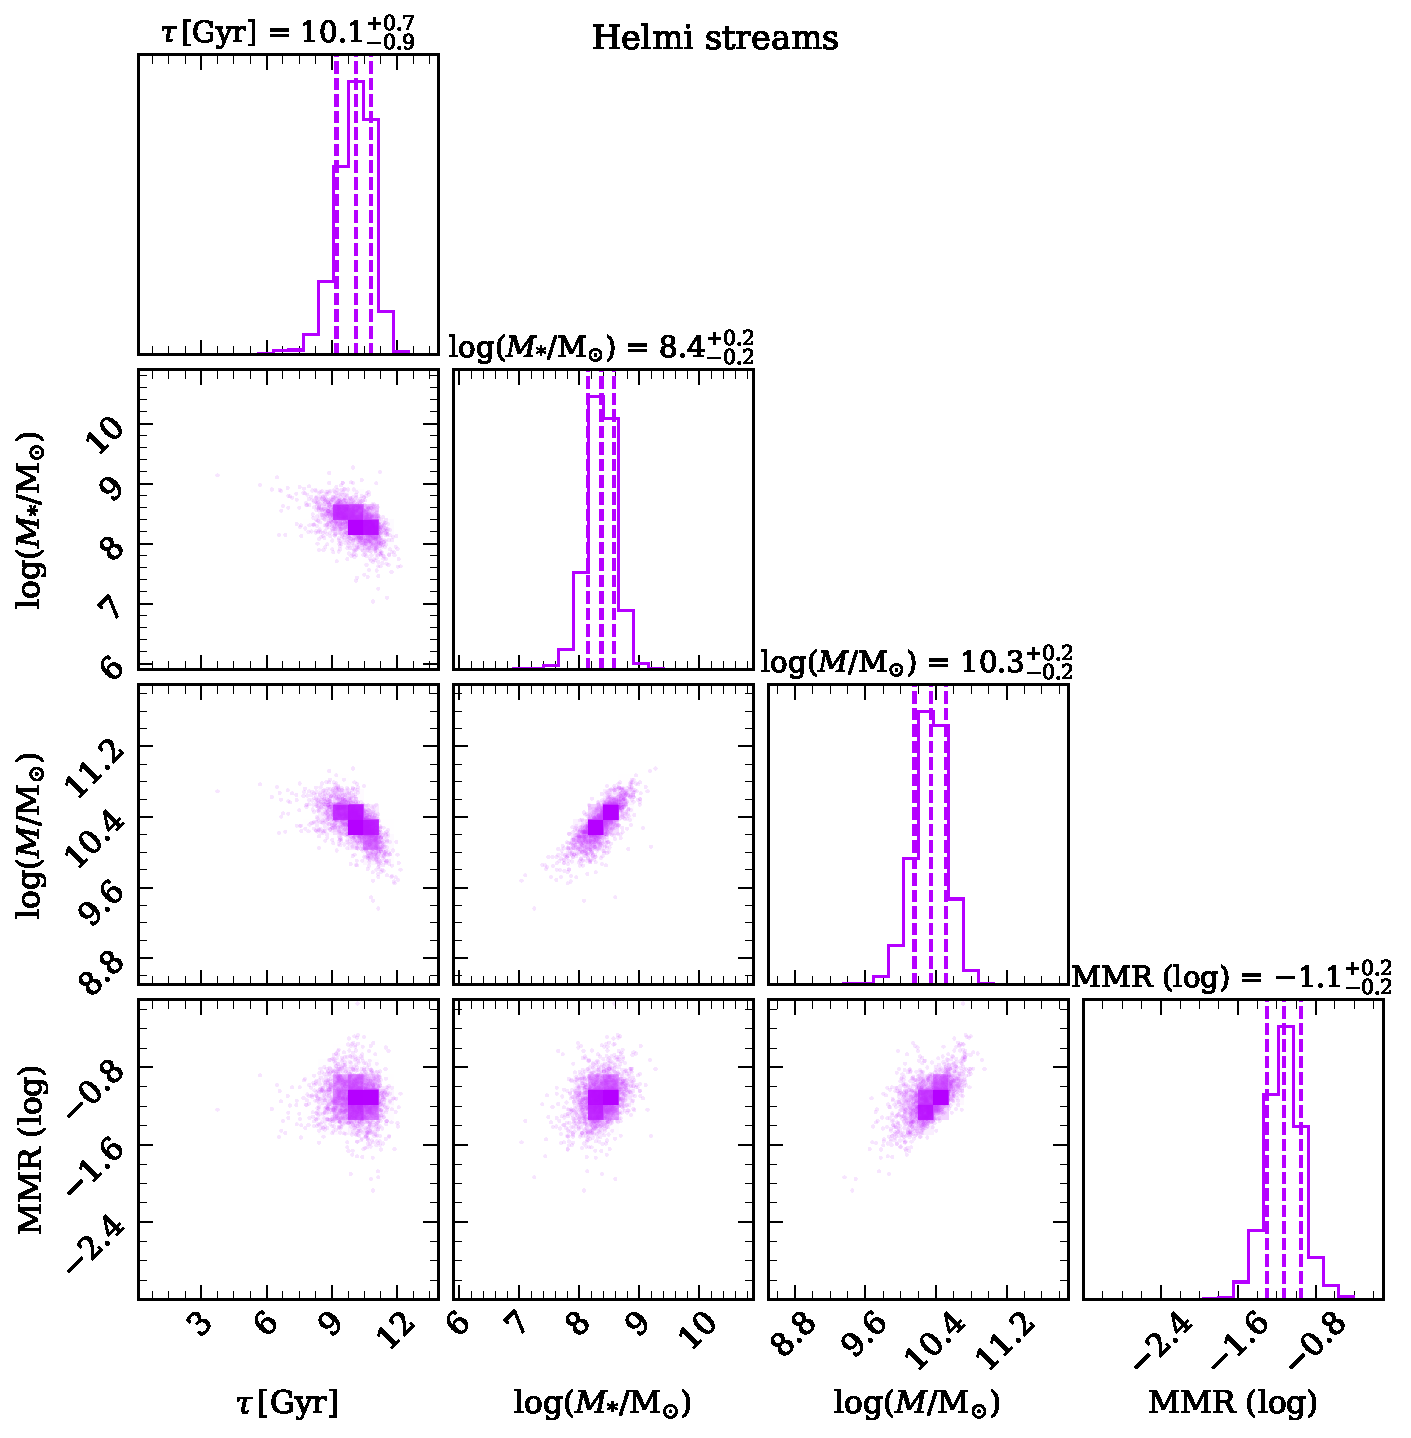
\includegraphics[width=\linewidth]{Helmi.pdf}
    \caption{}
    \label{fig:Helmi_pdf}
\end{figure*}

\begin{figure*}
    \centering
    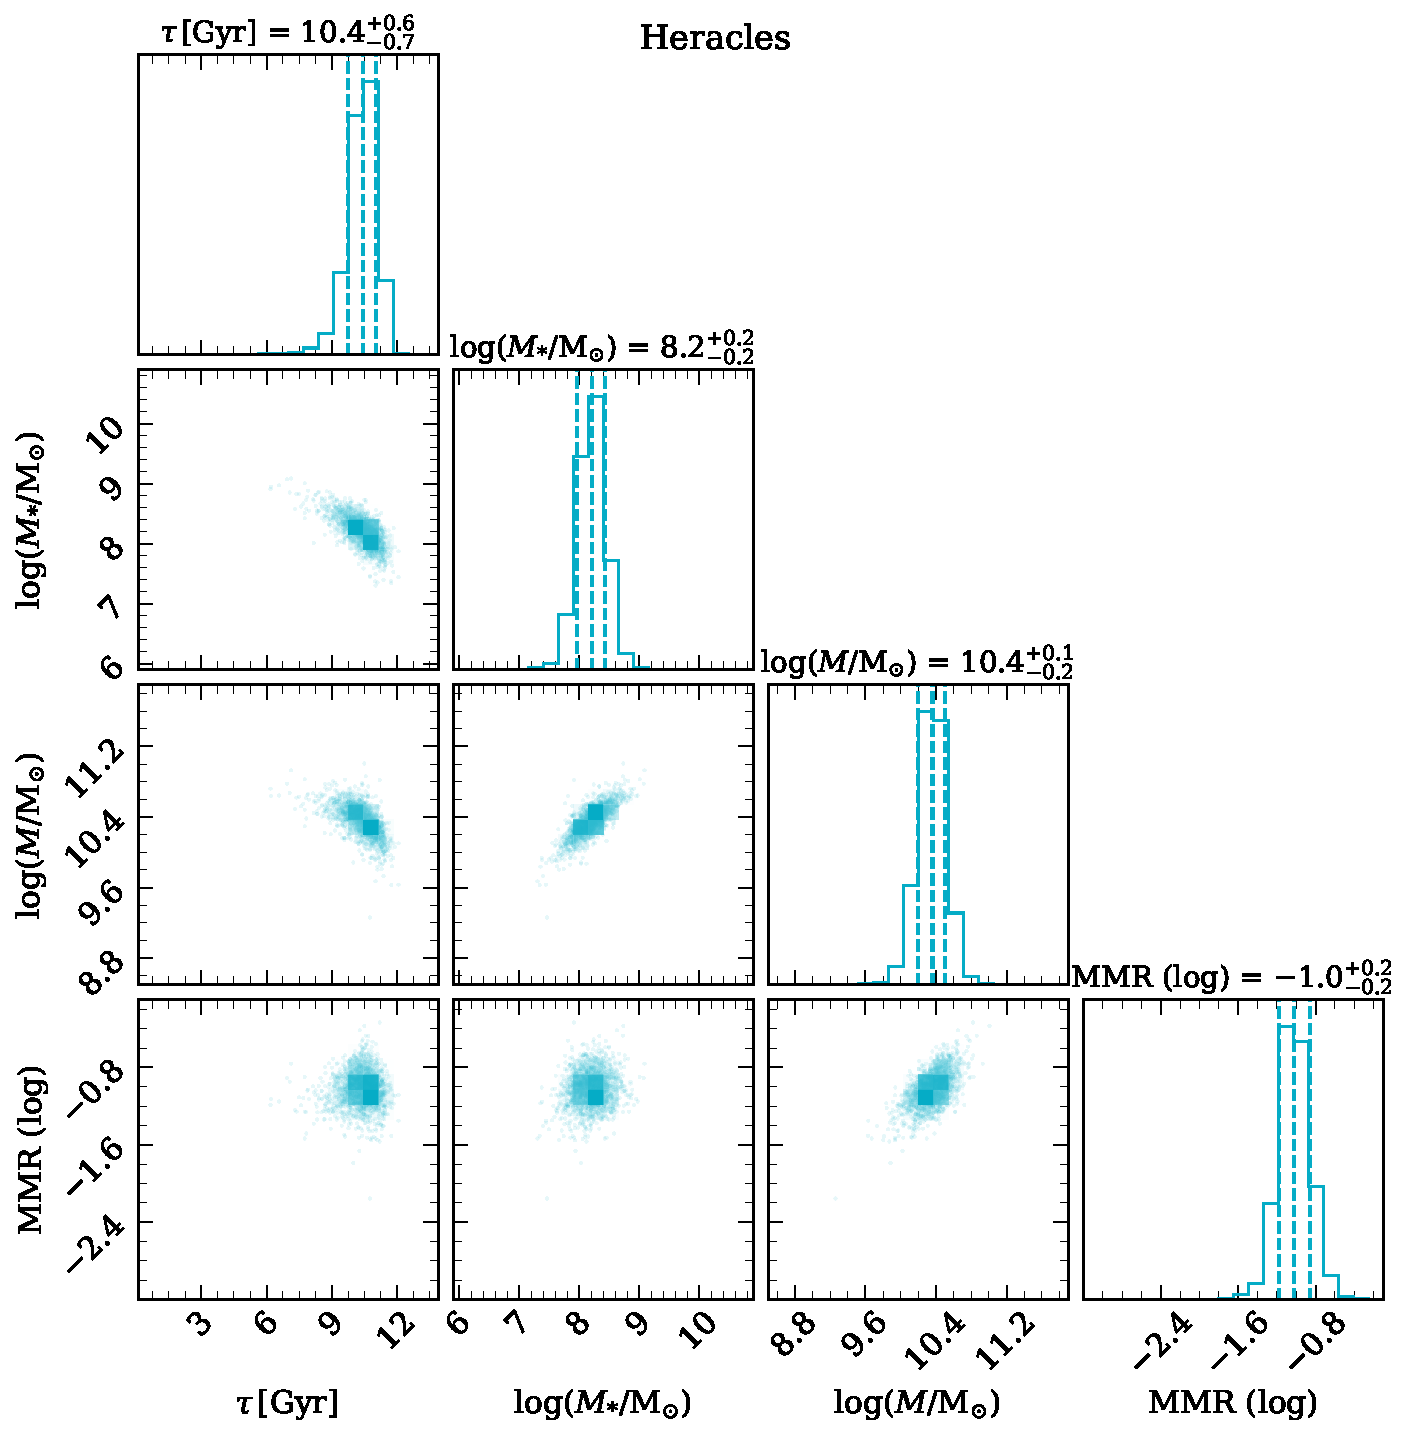
\includegraphics[width=\linewidth]{Heracles.pdf}
    \caption{}
    \label{fig:Heracles_pdf}
\end{figure*}

\begin{figure*}
    \centering
    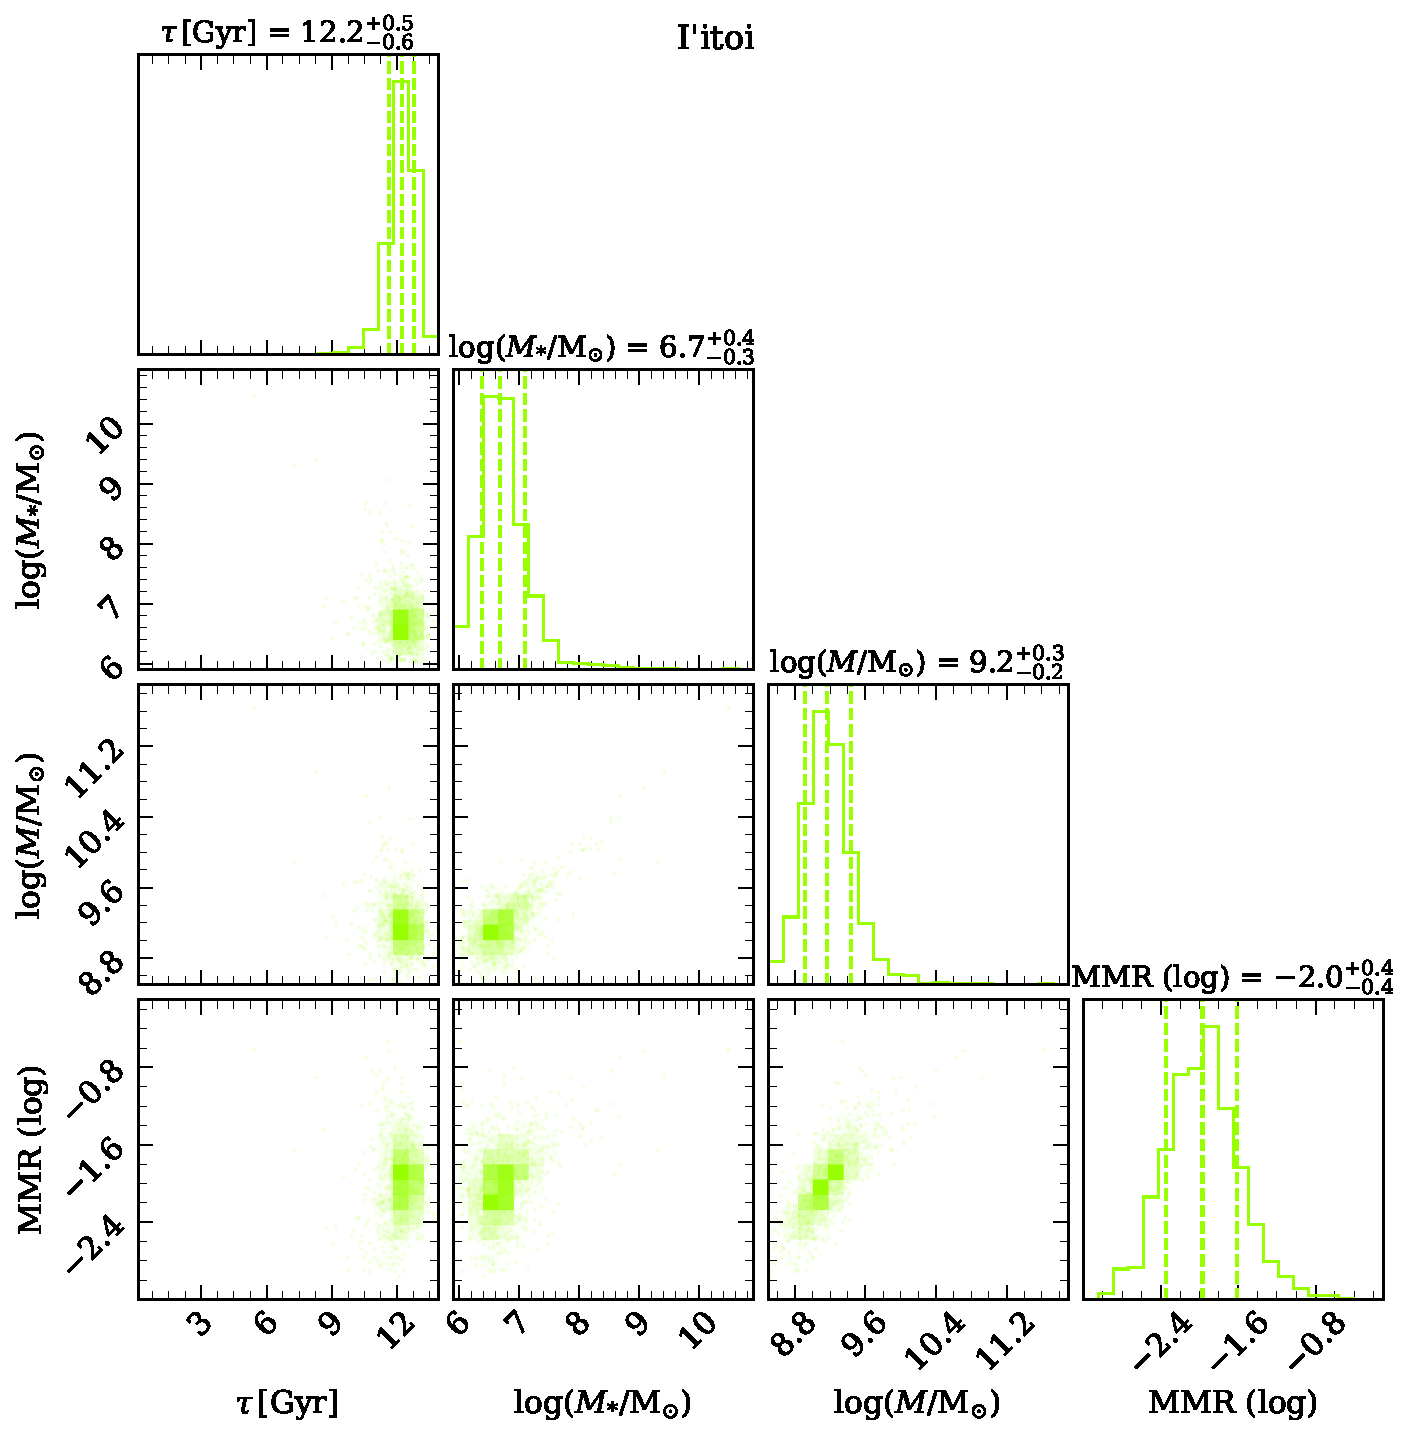
\includegraphics[width=\linewidth]{Iitoi.pdf}
    \caption{}
    \label{fig:Iitoi_pdf}
\end{figure*}

\begin{figure*}
    \centering
    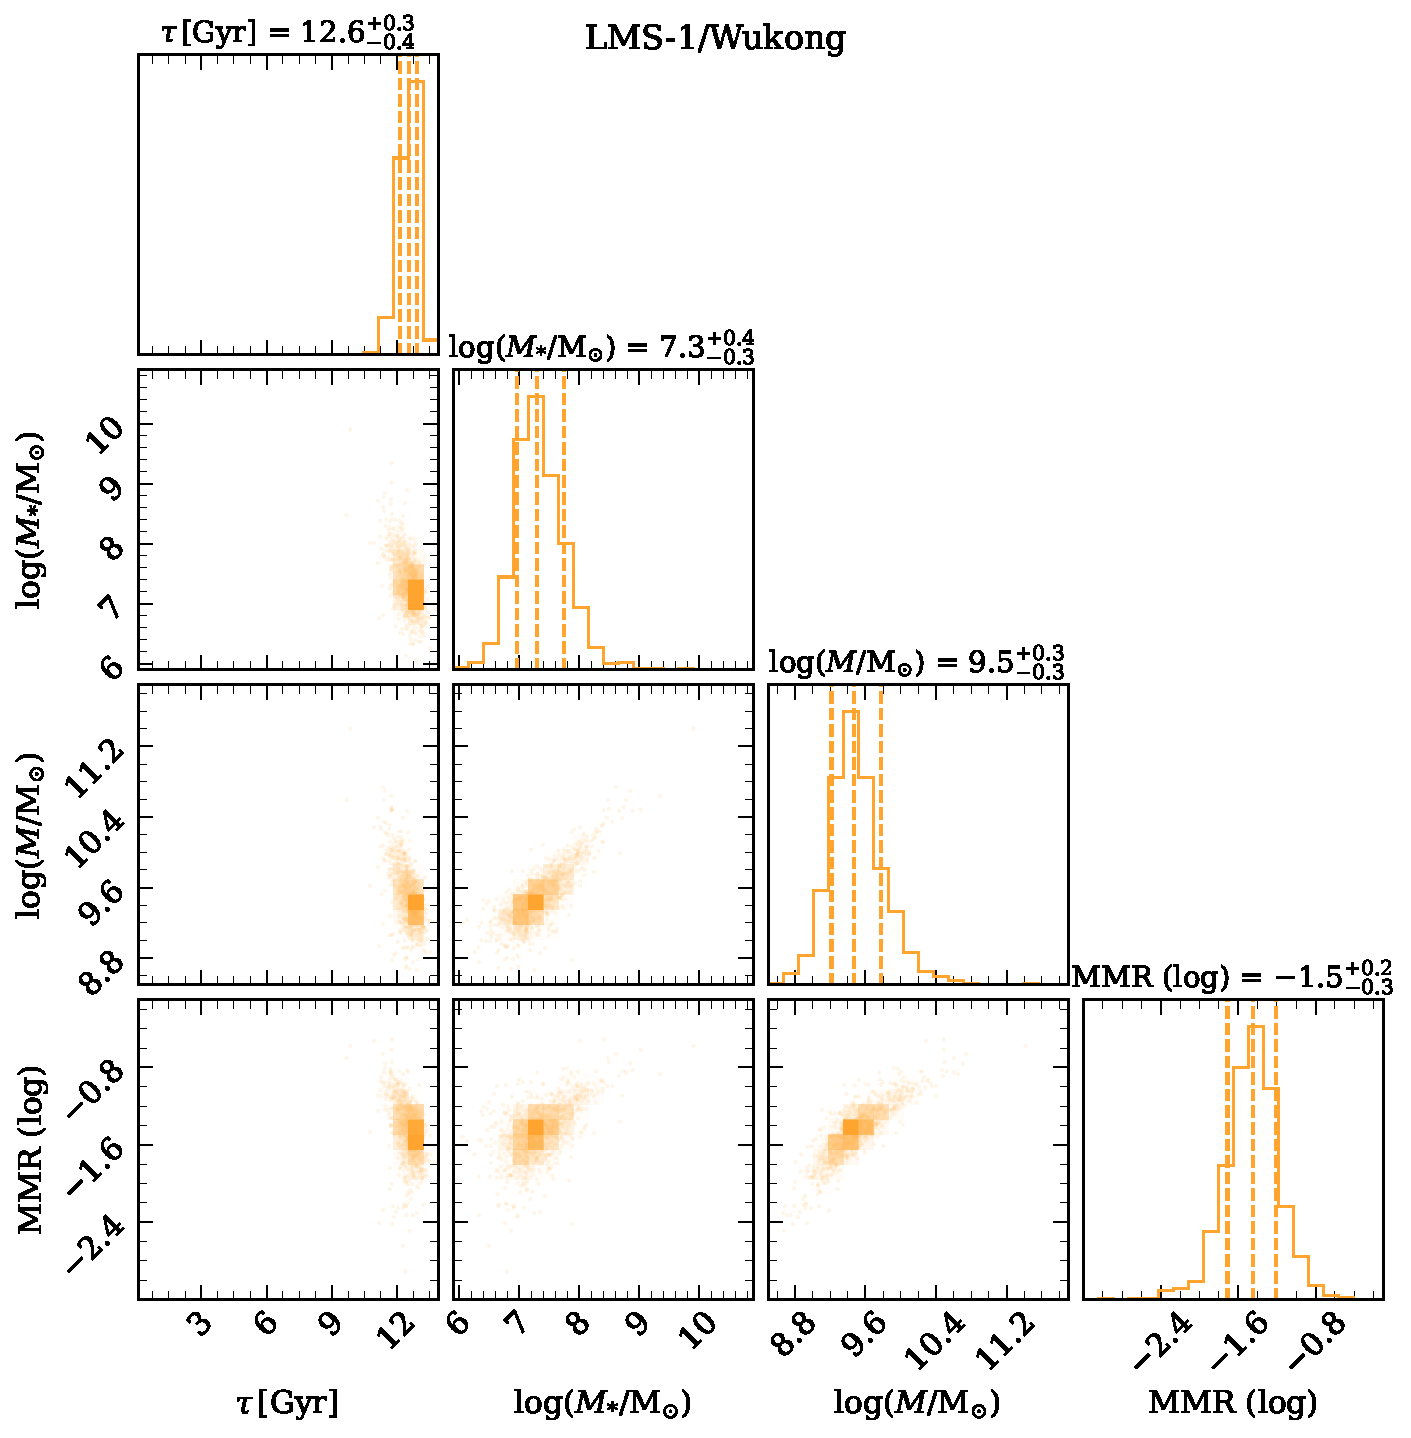
\includegraphics[width=\linewidth]{LMS.pdf}
    \caption{}
    \label{fig:LMS_pdf}
\end{figure*}

\begin{figure*}
    \centering
    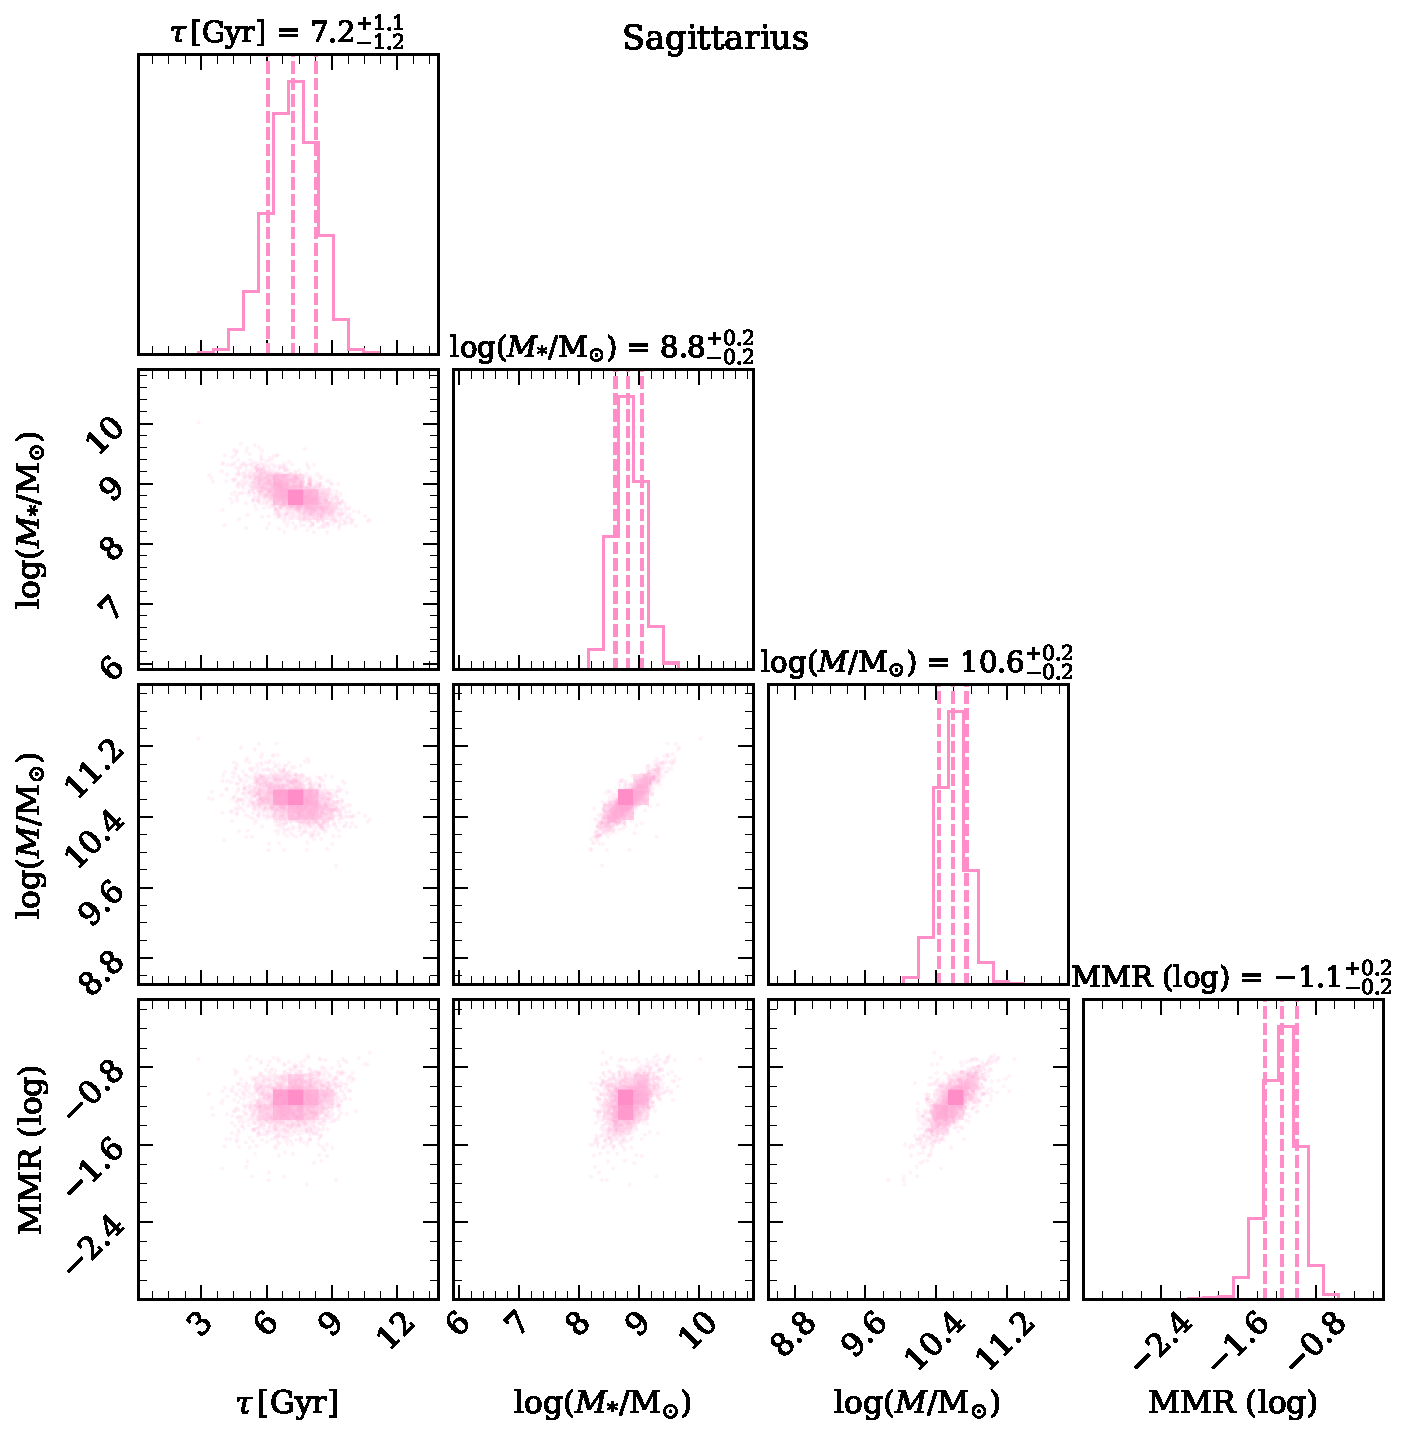
\includegraphics[width=\linewidth]{Sagittarius.pdf}
    \caption{}
    \label{fig:Sagittarius_pdf}
\end{figure*}

\begin{figure*}
    \centering
    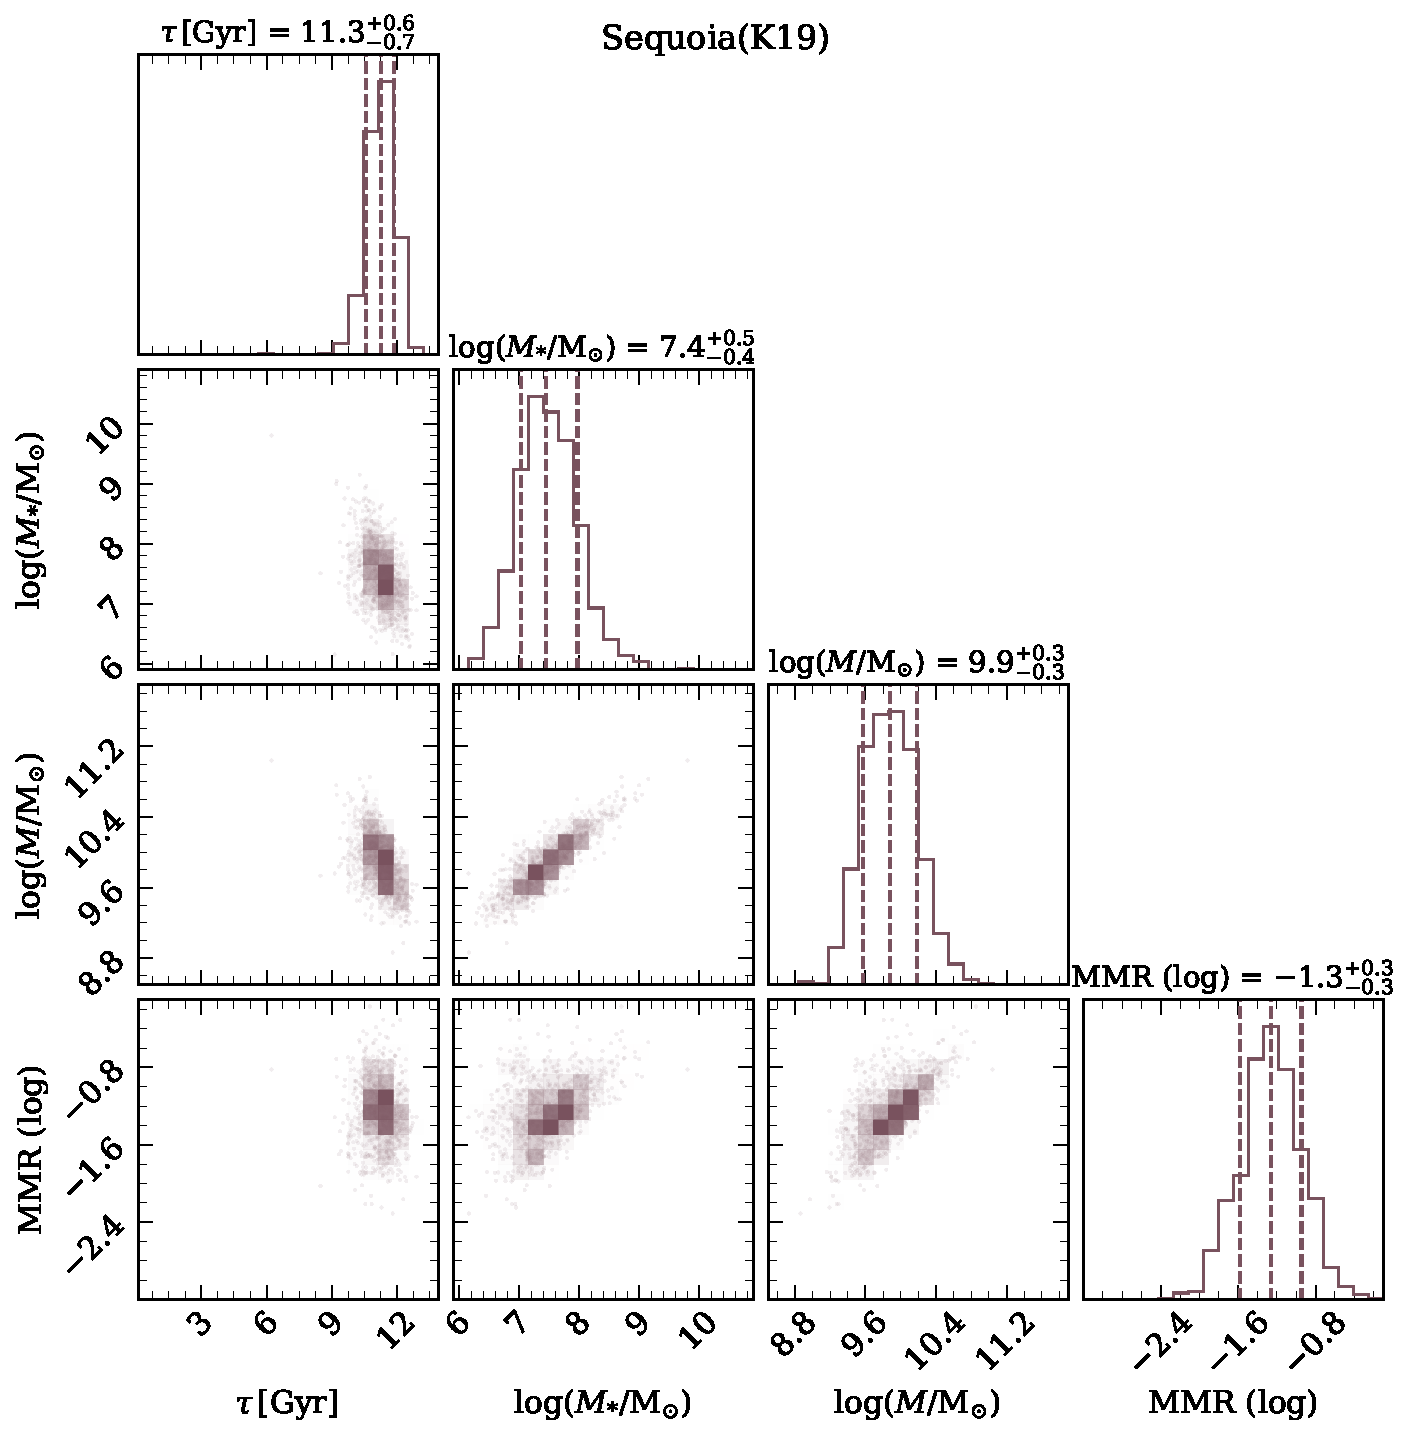
\includegraphics[width=\linewidth]{Sequoia_K19.pdf}
    \caption{}
    \label{fig:Sequoia_K19_pdf}
\end{figure*}

\begin{figure*}
    \centering
    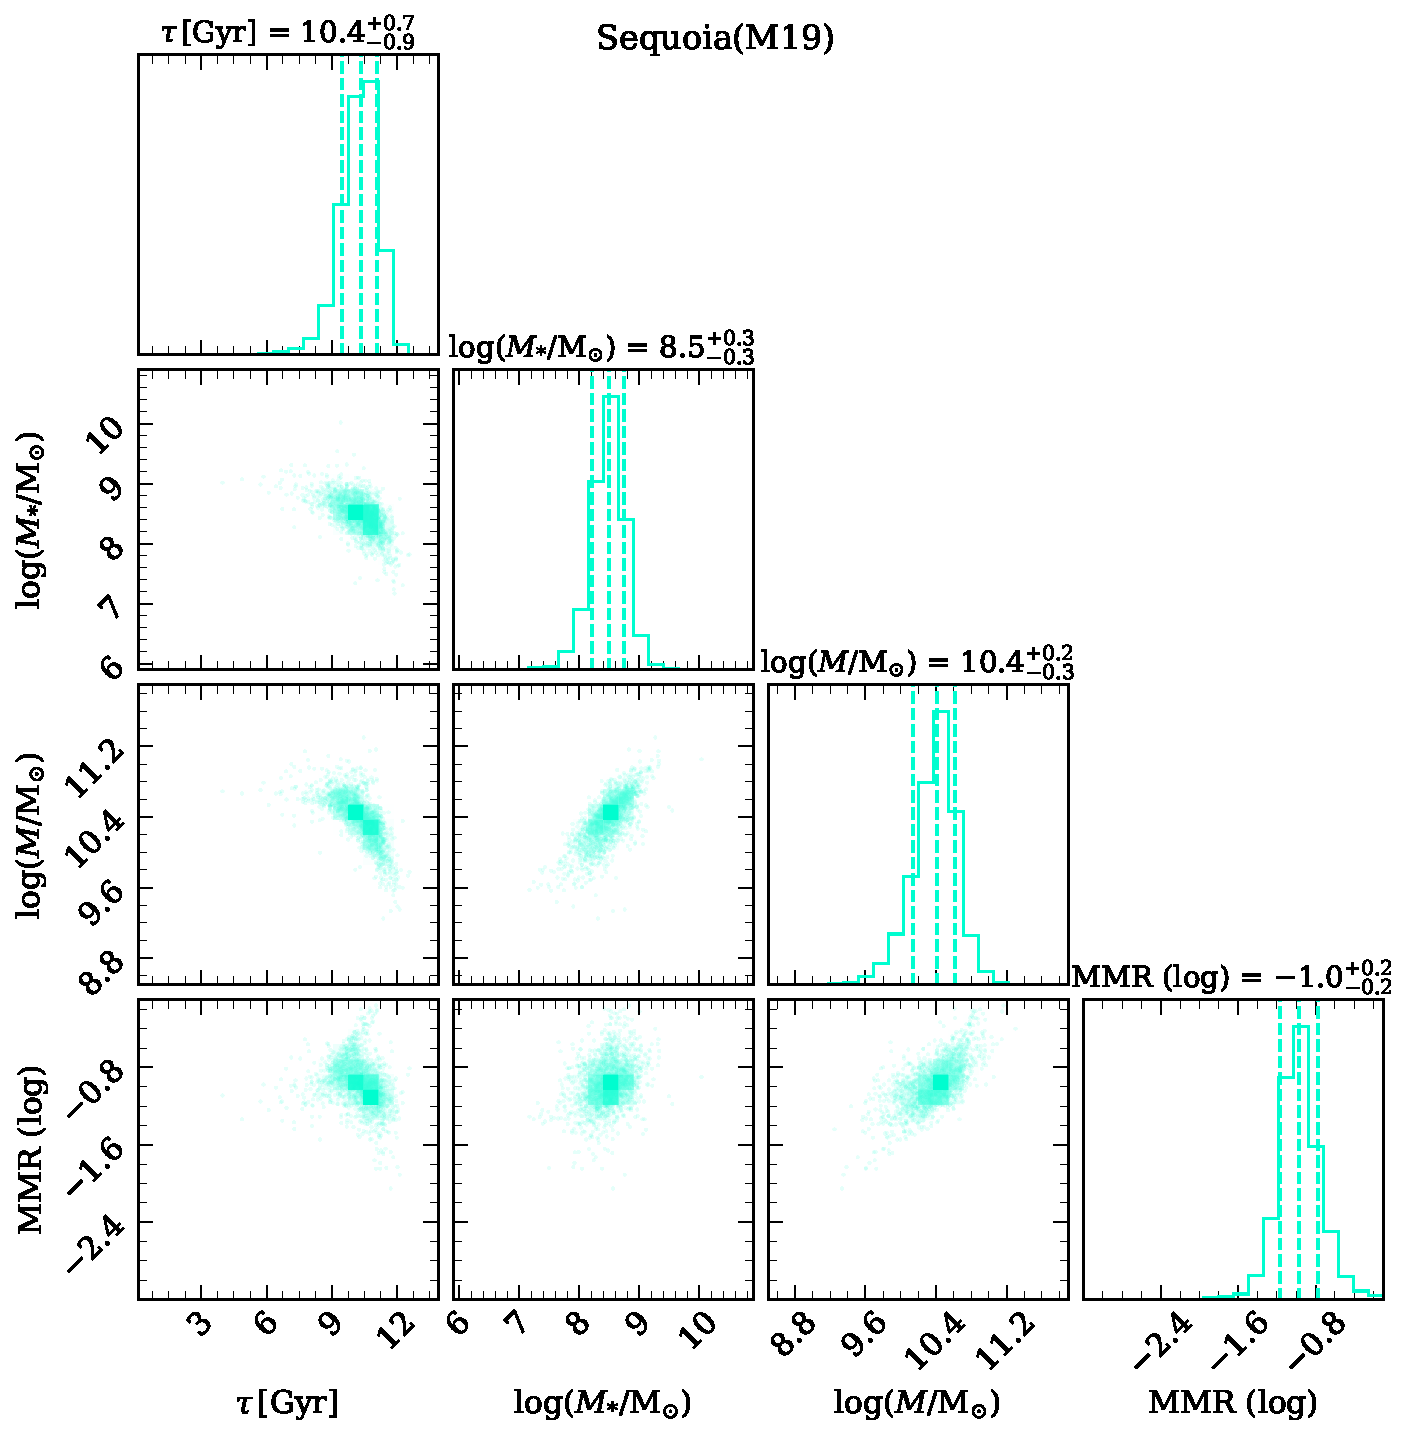
\includegraphics[width=\linewidth]{Sequoia_M19.pdf}
    \caption{}
    \label{fig:Sequoia_M19_pdf}
\end{figure*}

\begin{figure*}
    \centering
    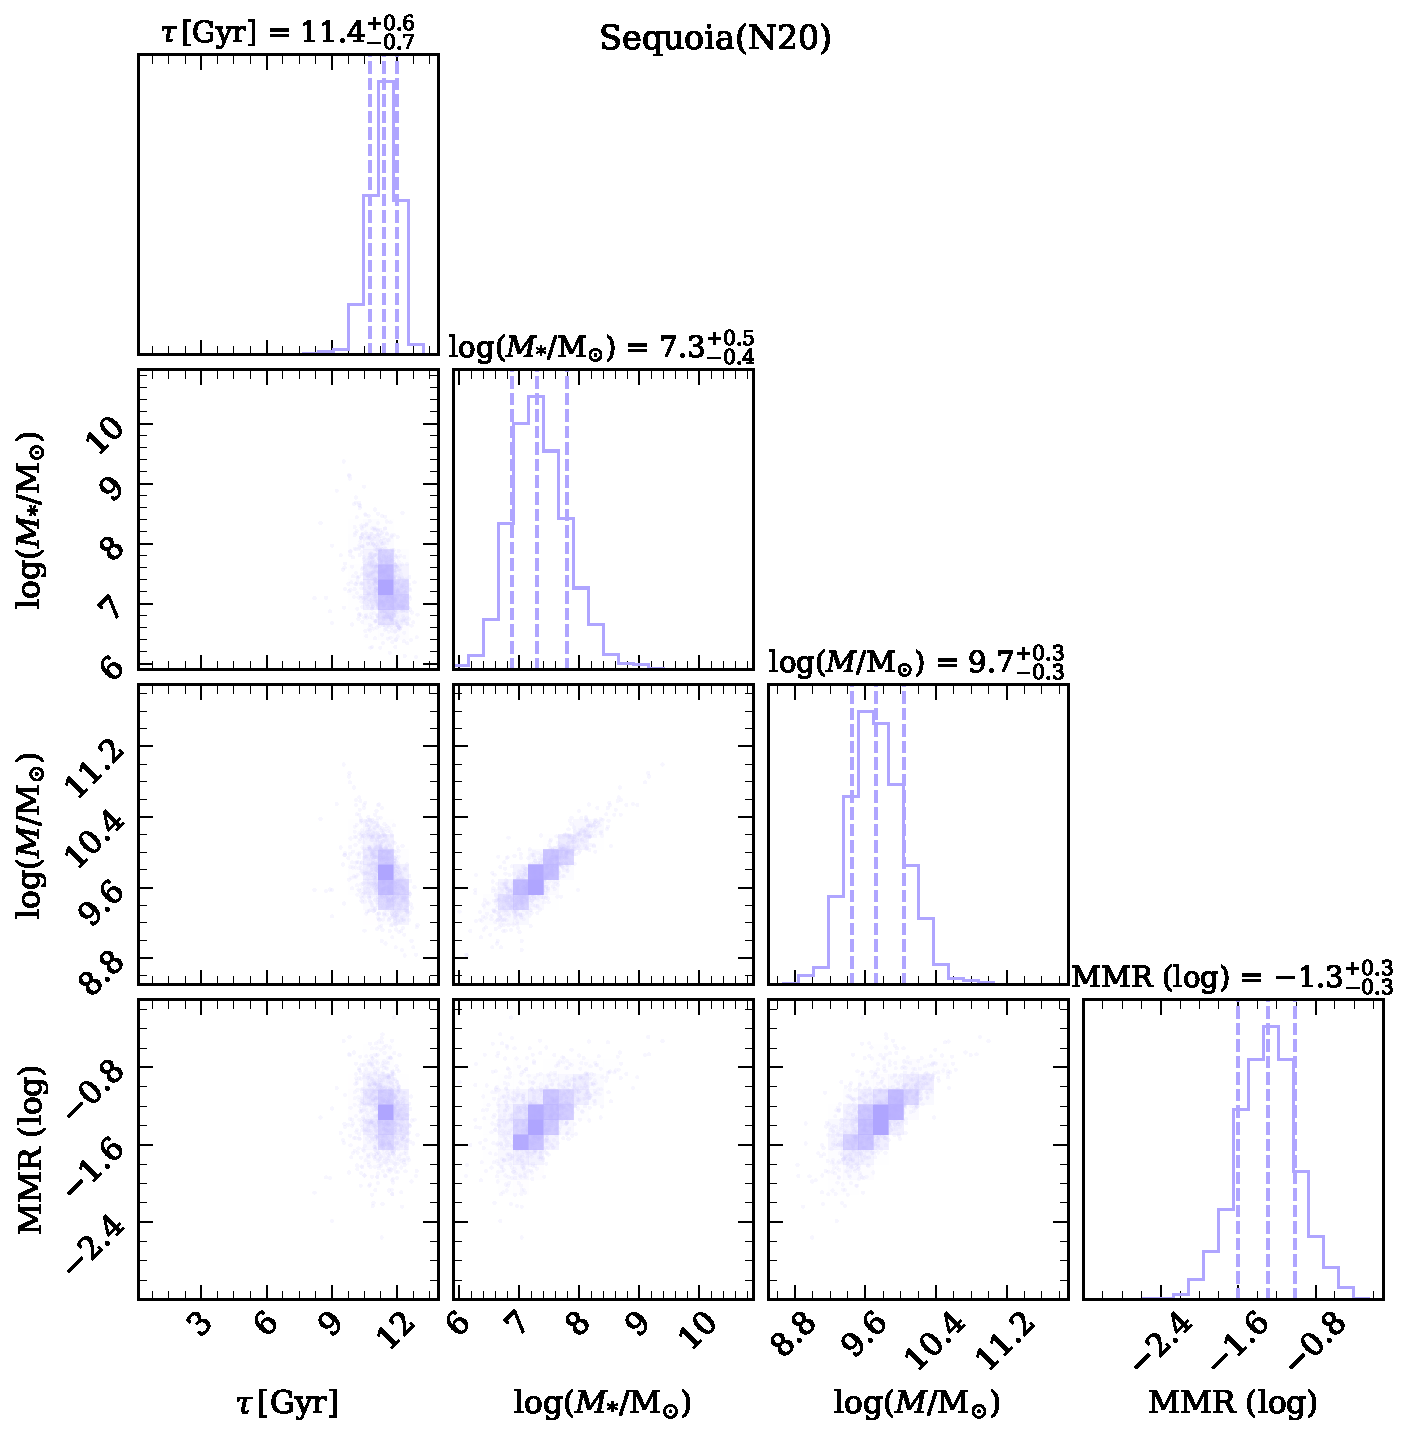
\includegraphics[width=\linewidth]{Sequoia_N20.pdf}
    \caption{}
    \label{fig:Sequoia_N20_pdf}
\end{figure*}

\begin{figure*}
    \centering
    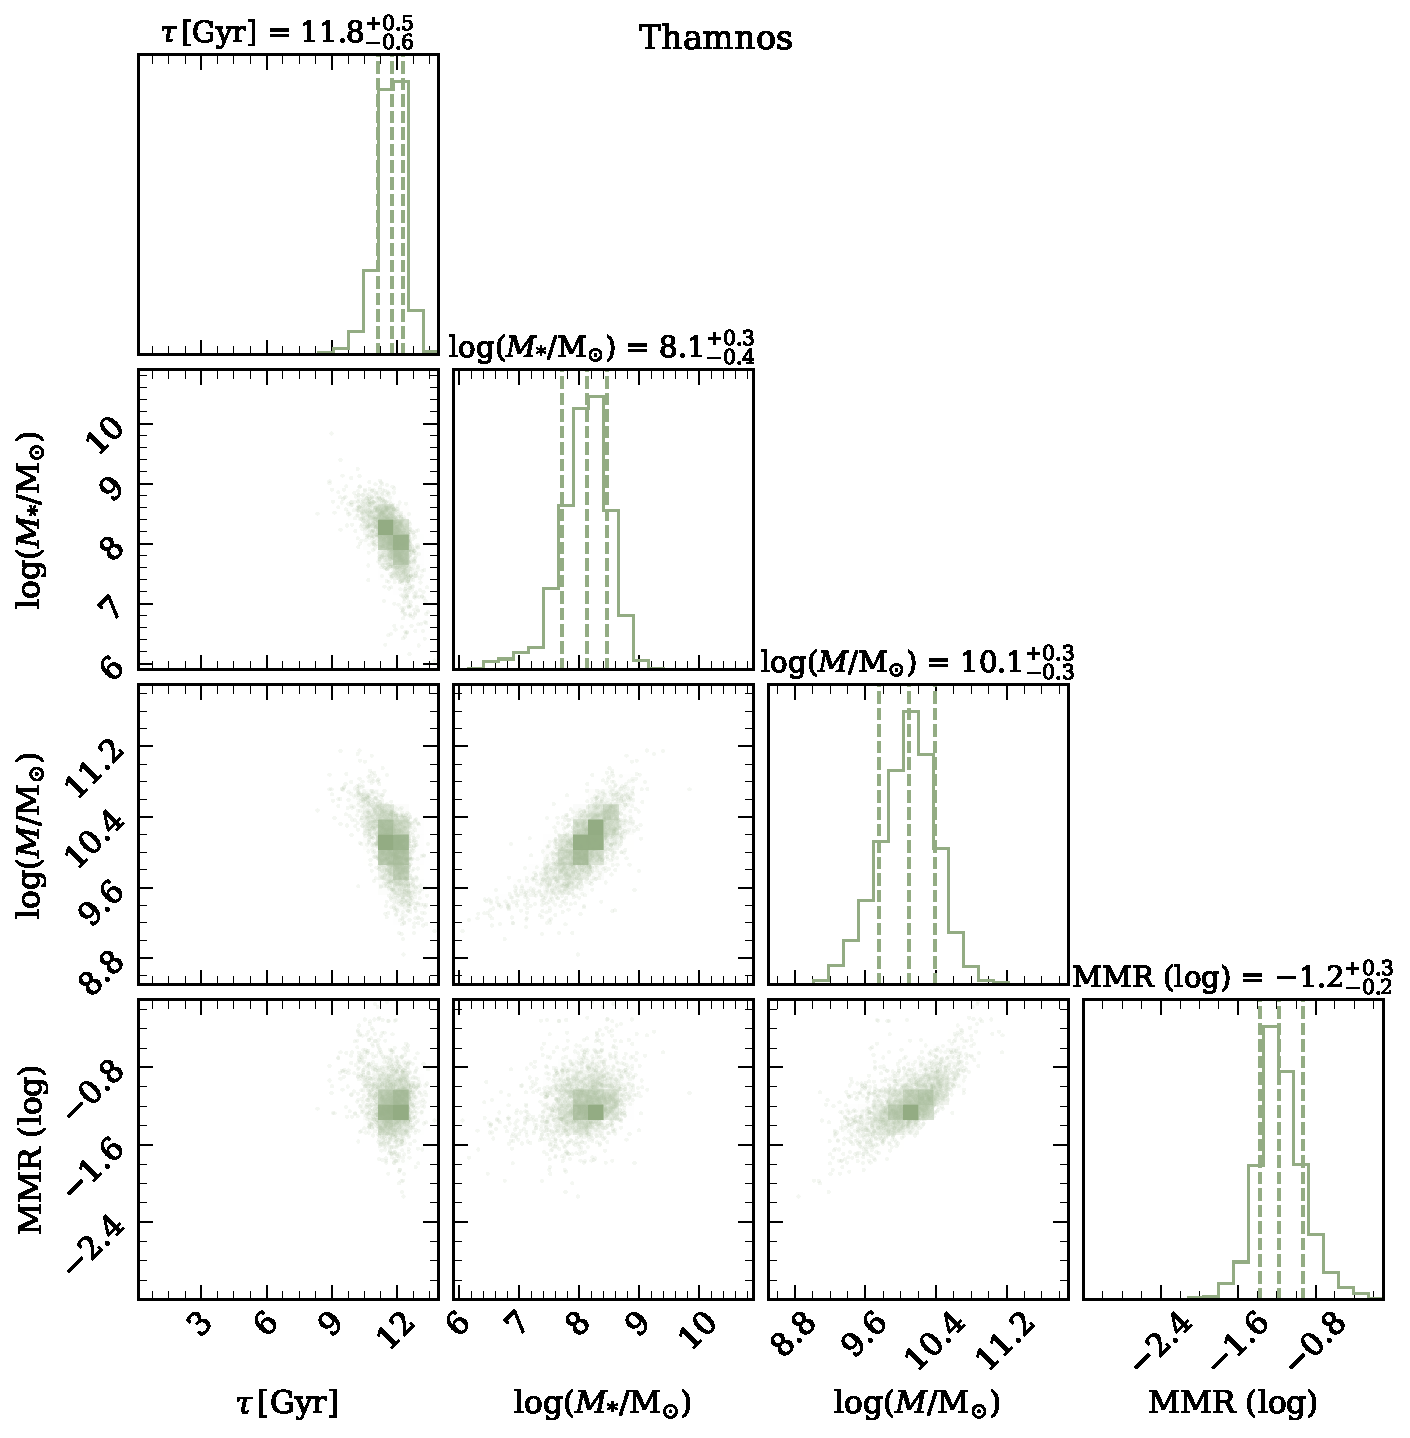
\includegraphics[width=\linewidth]{Thamnos.pdf}
    \caption{}
    \label{fig:Thamnos_pdf}
\end{figure*}
